\documentclass[a4paper,UTF8]{article}
\usepackage{ctex}
\usepackage[margin=1.25in]{geometry}
\usepackage{color}
\usepackage{graphicx}
\usepackage{amssymb}
\usepackage{amsmath}
\usepackage{amsthm}
\usepackage{enumerate}
\usepackage{bm}
\usepackage{hyperref}
\numberwithin{equation}{section}
%\usepackage[thmmarks, amsmath, thref]{ntheorem}
\theoremstyle{definition}
\newtheorem*{solution}{Solution}
\newtheorem*{prove}{Proof}
\newcommand{\indep}{\rotatebox[origin=c]{90}{$\models$}}

\usepackage{multirow}

%--

%--
\begin{document}
\title{机器学习导论\\
习题五}
\author{151250104, 卢以宁,  kiwiloveskiwis@gmail.com}
\maketitle
\section{[25pts] Bayes Optimal Classifier}
试证明在二分类问题中,但两类数据同先验、满足高斯分布且协方差相等时,LDA可产生贝叶斯最优分类器。
\begin{solution}
此处用于写证明(中英文均可)
~\\
~\\
~\\
\end{solution}

\section{[25pts] Naive Bayes}
考虑下面的400个训练数据的数据统计情况,其中特征维度为2($\mathbf{x}=[x_1,x_2]$),每种特征取值0或1,类别标记$y\in\{-1,+1\}$。详细信息如表\ref{table:training}所示。

根据该数据统计情况,请分别利用直接查表的方式和朴素贝叶斯分类器给出$\mathbf{x}=[1,0]$的测试样本的类别预测,并写出具体的推导过程。
\begin{table}[h]
\centering
\caption{数据统计信息}
\label{table:training}\vspace{2mm}
\begin{tabular}{cc|cc}\hline
$x_1$		&  $x_2$ 	&	$y=+1$	&	$y=-1$ 	\\ \hline
0		&  0 	&	90	&	10 \\
0		&  1 	&	90 	&	10 \\
1		&  0 	&	51 	&	49 \\
1		&  1 	&	40 	&	60 \\\hline
\end{tabular}
\end{table}

\begin{solution}
此处用于写解答(中英文均可)
~\\
~\\
~\\
\end{solution}

\section{\textbf{[25pts]} Bayesian Network}
贝叶斯网(Bayesian Network)是一种经典的概率图模型,请学习书本7.5节内容回答下面的问题:

(1) \textbf{[5pts]} 请画出下面的联合概率分布的分解式对应的贝叶斯网结构:
\begin{equation*}
\Pr(A, B, C, D, E, F) = \Pr(A)\Pr(B)\Pr(C)\Pr(D|A)\Pr(E|A)\Pr(F|B, D)\Pr(G|D, E)
\end{equation*}

(2) \textbf{[5pts]} 请写出图\ref{fig-DAG}中贝叶斯网结构的联合概率分布的分解表达式。
\begin{figure}[h]
\label{fig-DAG}
\centering
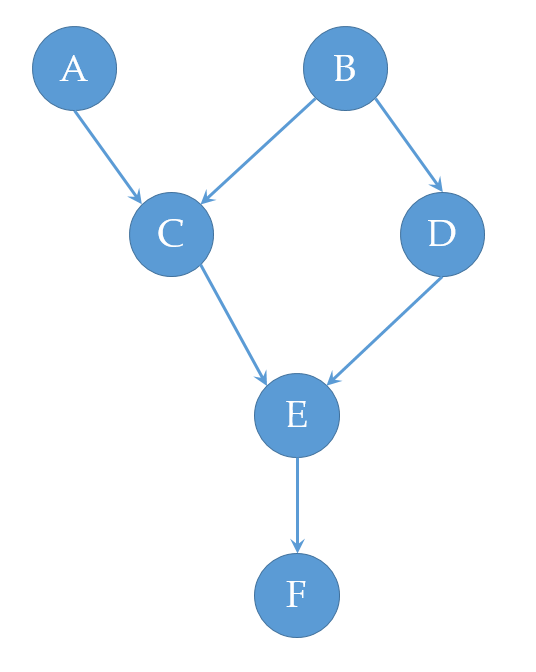
\includegraphics[scale=0.3]{bayes_net.png}
\caption{题目3-(2)有向图}
\end{figure}

(3) \textbf{[15pts]} 基于第(2)问中的图\ref{fig-DAG}, 请判断表格\ref{table:DAG}中的论断是否正确,只需将下面的表格填完整即可。
\begin{table}[h]
\centering
\caption{判断表格中的论断是否正确}
\label{table:DAG}
\begin{tabular}{c|l|c||c|l|c}\hline
序号   		& 		关系  			& True/False 	& 序号   	& 		关系  			& True/False \\ \hline
1			&	$A \indep B$ 		    & 			    & 7  		& 	$F \indep B|C$ 		& 			 \\
2			&	$A \indep B|C$ 	    & 			    & 8  		& 	$F \indep B|C, D$ 	& 			 \\
3			&	$C \indep D $		    & 			    & 9  		& 	$F \indep B|E$ 		& 			 \\
4			&	$C \indep D|E$ 	    & 			    & 10  		& 	$A \indep F $			& 			 \\
5			&	$C \indep D|B, F$     & 			    & 11  		& 	$A \indep F|C$ 		& 			 \\
6			&	$F \indep B $		    & 			    & 12  		& 	$A \indep F|D$ 		& 			 \\ \hline
\end{tabular}
\end{table}

\begin{solution}
此处用于写解答(中英文均可)
~\\
~\\
~\\
\end{solution}


\section{[25pts] Naive Bayes in Practice}
请实现朴素贝叶斯分类器,同时支持离散属性和连续属性。详细编程题指南请参见链接:\url{http://lamda.nju.edu.cn/ml2017/PS5/ML5_programming.html}. 

同时,请简要谈谈你的感想。实践过程中遇到了什么问题,你是如何解决的?
\begin{solution}
此处用于写解答(中英文均可)
~\\
~\\
~\\
\end{solution}
\end{document}